\documentclass[11pt]{article}
\usepackage{latexsym}
\usepackage{amssymb}
\usepackage{times}
%\usepackage[in]{fullpage}
\usepackage{amsmath,amsfonts,amsthm}
\usepackage{array}
\usepackage{multirow}
\usepackage{tikz}
\usepackage{enumitem}
\usepackage{graphicx}


\oddsidemargin 0mm
\evensidemargin 5mm
\topmargin -20mm
\textheight 240mm
\textwidth 160mm

%\documentclass[11pt]{article}
%\pagestyle{myheadings}
%\usepackage[ruled,nothing]{algorithm}
%\usepackage{algorithmic}
%\usepackage[dvips]{epsfig,graphicx}
%\numberwithin{equation}{section}

\newenvironment{newalgo}[2]{\begin{algorithm}

\caption{\textsc{#1}}\label{#2}

\begin{algorithmic}[1]}{\end{algorithmic}\end{algorithm}}

\newcommand\MyBox[2]{
  \fbox{\lower0.75cm
    \vbox to 1.7cm{\vfil
      \hbox to 1.7cm{\hfil\parbox{1.4cm}{#1\\#2}\hfil}
      \vfil}%
  }%
}

\newcommand{\gm}{\gamma}
\newcommand{\wh}{\widehat}
\newcommand{\rep}{representation}
\newcommand{\rv}{random variable}
\newcommand{\la}{\lambda}
\newcommand{\wt}{\widetilde}
\newcommand{\st}{such that}
\newcommand{\slvary}{slowly varying}
\newcommand{\ma}{moving average}
\newcommand{\regvary}{regularly varying}
\newcommand{\asy}{asymptotic}
\newcommand{\ts}{time series}
\newcommand{\id}{infinitely divisible}
\newcommand{\seq}{sequence}
\newcommand{\fidi}{finite dimensional \ds}

\newcommand{\ble}{\begin{lemma}}
\newcommand{\ele}{\end{lemma}}
\newcommand{\bfX}{{\bf X}}
\newcommand{\pro}{probabilit}
\newcommand{\BX}{{\bf X}}
\newcommand{\BY}{{\bf Y}}
\newcommand{\BZ}{{\bf Z}}
\newcommand{\BV}{{\bf V}}
\newcommand{\BW}{{\bf W}}
\newcommand{\reals}{{\mathbb R}}
\newcommand{\bbr}{\reals}

\newcommand{\balpha}{\mbox{\boldmath$\alpha$}}
\newcommand{\bbeta}{\mbox{\boldmath$\beta$}}
\newcommand{\bmu}{\mbox{\boldmath$\mu$}}
\newcommand{\tbmu}{\mbox{\boldmath${\tilde \mu}$}}
\newcommand{\bEta}{\mbox{\boldmath$\eta$}}


\def \br#1{\left \{#1 \right \}}
\def \pr#1{\left (#1 \right)}

\newcommand{\Gm}{\Gamma}
\newcommand{\ep}{\epsilon}


\newtheorem{lemma}{Lemma}[section]
\newtheorem{figur}[lemma]{Figure}
\newtheorem{theorem}[lemma]{Theorem}
\newtheorem{proposition}[lemma]{Proposition}
\newtheorem{definition}[lemma]{Definition}
\newtheorem{corollary}[lemma]{Corollary}
\newtheorem{example}[lemma]{Example}
\newtheorem{exercise}[lemma]{Exercise}
\newtheorem{remark}[lemma]{Remark}
\newtheorem{fig}[lemma]{Figure}
\newtheorem{tab}[lemma]{Table}
\newtheorem{fact}[lemma]{Fact}
\newtheorem{test}{Lemma}
\newtheorem{algorithm}[lemma]{Algorithm}

\newcommand{\play}{\displaystyle}

\newcommand{\ms}{measure}
\newcommand{\beao}{\begin{eqnarray*}}
\newcommand{\eeao}{\end{eqnarray*}\noindent}
\newcommand{\beam}{\begin{eqnarray}}
\newcommand{\eeam}{\end{eqnarray}\noindent}

\newcommand{\halmos}{\hfill\mbox{\qed}\\}
\newcommand{\fct}{function}
\newcommand{\ins}{insurance}

\newcommand{\one}{{\bf 1}}
\newcommand{\eid}{\buildrel{\rm d}\over {=}}
\newcommand {\Or}{\rm ORDER}
\newcommand {\In}{\rm INTER}

\newcommand{\bbd}{{\mathbb D}}
\newcommand{\vi}{$V_{ij}$ }
\newcommand{\rr}{R^{\prime\prime}}
%\newcommand{\R}{R^\prime}
\newcommand{\ci}{\frac{1}{c}}
\newcommand{\Vi}{V(n)}
\newcommand{\dR}{\mathcal R}
\newcommand{\md}[1]{\left(\ \rm{mod}\ \it{#1}\right)}
\newcommand{\So}{s}
\usepackage{algpseudocode, caption}
\usepackage[ruled]{algorithm}
%\begin{document}
%\def\DoubleSpace{\baselineskip=24pt}
%\DoubleSpace \sloppy

\begin{document}


\title{Modulo7 Status Report : Progress of Master's Essay}
\author{\textbf{Arunav Sanyal}}

\maketitle

%%%%%%%%%%%%%%%%%%%%%%%%%%%%%%%%%%

\section*{Code and Design Level Progress}

\begin{enumerate}
\item Implemented basic similarity measures and vector space models for polyphonic and Monophonic Music. These vector space models are based on expressions of pitch, rhythm and overall charecteristics like pitch duration
\item Implemented a templated based key signature algorithm
\item Completed feature extraction from all Music sources and sanity tested them.
\item Completed database internal database creation. 
\item Completing indexing lyrics based on document frequency and songs on metadata terms
\item \textbf{Next phase:} Work on more similarity measures and estimate precision and recall on ground truth data. Work on time signature estimation algorithm \textbf{ETA : 28 September 2015}
\item \textbf{Further direction of work:} Design SQL like query system for Modulo7 \textbf{ETA : 15 October 2015}
\end{enumerate}


\section*{Experimental Progress}

\begin{enumerate}
\item Completed acquisition of certain small published datasets for analysis.
\item Completed test cases on indexing on key signature and time signature. Given presence of key and time signature in encoding, tested correctness of program.
\item Completed testing compression factor Modulo7 from midi and mp3 sources (while preserving core symbolic information. This data is for 50 tracks which are encoded in midi and mp3 and converted into the Modulo7 format. Attached bar graph for your perusal on the next page. Results are positive and as expected. 
\item \textbf{Complete compression factor test cases for all sources} Design and run test cases for similarity measures. \textbf{ETA : 28 September 2015}
\item \textbf{Further direction of work:} Run test cases on the million song dataset. 
\textbf{This would require CPU cycles on CLSP servers so I will require permission} \textbf{ETA : 30 October 2015}
 
\begin{figure}
\centering
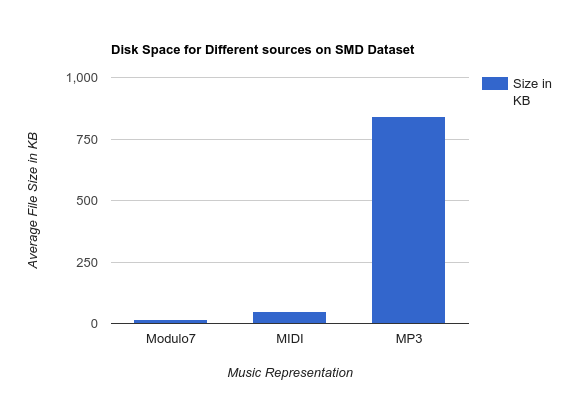
\includegraphics[width=\textwidth]{Modulo7SMDBarGraph.png}
\makeatletter
\let\@currsize\normalsize
\caption{Modulo7 architectural design}
\label{fig:figure}
\end{figure}


\end{enumerate}
\end{document}

%%%%%%%%%%%%%%%%%%%%%%%%%%%%%
